% allgem. Dokumentenformat
\documentclass[a4paper,12pt,headsepline,twocolumn]{scrartcl}

% weitere Pakete
% Grafiken aus PNG Dateien einbinden
\usepackage{graphicx}

%deletes first blank page
\usepackage{atbegshi}% http://ctan.org/pkg/atbegshi
\AtBeginDocument{\AtBeginShipoutNext{\AtBeginShipoutDiscard}}

%for links 
\usepackage{color}
\usepackage{hyperref}
\hypersetup{
    colorlinks=true,
    linkcolor=blue,
    urlcolor=red,
    linktoc=all
}
\usepackage{xr}
\externaldocument{Julian.tex}

% Deutsche Sonderzeichen benutzen 
%\usepackage{ngerman}

% deutsche Silbentrennung
\usepackage[ngerman]{babel}

% Eurozeichen einbinden
\usepackage[right]{eurosym}

% Umlaute unter UTF8 nutzen
\usepackage[utf8]{inputenc}

% Zeichenencoding
\usepackage[T1]{fontenc}

\usepackage{lmodern}
\usepackage{fix-cm}

% floatende Bilder ermöglichen
%\usepackage{floatflt}

% mehrseitige Tabellen ermöglichen
\usepackage{longtable}

% Unterstützung für Schriftarten
%\newcommand{\changefont}[3]{ 
%\fontfamily{#1} \fontseries{#2} \fontshape{#3} \selectfont}

% Packet für Seitenrandabständex und Einstellung für Seitenränder
\usepackage{geometry}
\geometry{left=3.5cm, right=2cm, top=2.5cm, bottom=2cm}

% Paket für Boxen im Text
\usepackage{fancybox}

% bricht lange URLs "schoen" um
%\usepackage[hyphens,obeyspaces,spaces]{url}

% Paket für Textfarben
\usepackage{color}

% Mathematische Symbole importieren
\usepackage{amssymb}

% neue Kopfzeilen mit fancypaket
\usepackage{fancyhdr} %Paket laden
\pagestyle{fancy} %eigener Seitenstil
\fancyhf{} %alle Kopf- und Fußzeilenfelder bereinigen
\fancyhead[L]{\nouppercase{\leftmark}} %Kopfzeile links
\fancyhead[C]{} %zentrierte Kopfzeile
\fancyhead[R]{\thepage} %Kopfzeile rechts
\renewcommand{\headrulewidth}{0.4pt} %obere Trennlinie
%\fancyfoot[C]{\thepage} %Seitennummer
%\renewcommand{\footrulewidth}{0.4pt} %untere Trennlinie

% für Tabellen
\usepackage{array}

% Runde Klammern für Zitate
%\usepackage[numbers,round]{natbib}

% Festlegung Art der Zitierung - Havardmethode: Abkuerzung Autor + Jahr
\bibliographystyle{alphadin}

% Schaltet den zusätzlichen Zwischenraum ab, den LaTeX normalerweise nach einem Satzzeichen einfügt.
\frenchspacing

% Paket für Zeilenabstand
\usepackage{setspace}

% für Code-Listings
\usepackage{listings}

% für Bildbezeichner
\usepackage{capt-of}
\makeindex
\begin{document}
	
% Leere Seite am Anfang
\newpage
\thispagestyle{empty} % erzeugt Seite ohne Kopf- / Fusszeile
\section*{ }

%Titelseite

\begin{titlepage}
		
		\centering
		
\includegraphics[width=0.55\textwidth]{unistuttgart_logo_deutsch}\par\vspace{1cm}
		{\scshape\Large Bachelorforschungsprojekt Informatik\par}
		\vspace{1.5cm}
		{\huge\bfseries Entwicklung eines
			Online-Self-Assessment-Tests für
			Studieninteressenten der Universität Stuttgart\par}
		\vspace{2cm}
		{\Large\itshape Jonas Allali\par}
		\vspace{0.2cm}
		{\Large\itshape Julian Blumenröther\par}
		\vspace{0.2cm}
		{\Large\itshape Tim-Julian Ehret\par}
		\vspace{0.2cm}
		{\Large\itshape Sokol Makolli\par}
		\vspace{0.2cm}
		{\Large\itshape Jena Satkunarajan\par}
		\vspace{1cm}
		{\Large Prüfer: \par
			\vspace{0.3cm}
		\textsc{Prof. Dr.-Ing. Stefan Funke}}
		
		\vfill
		
		% Bottom of the page
		{\large \today\par}
\end{titlepage}	
\tableofcontents
% inkludiere einzelne Abschnitte
\clearpage

\section*{Kurzfassung}
\label{Abstract}
In dieser Arbeit wurde ein webunterstützender Self-Assessment-Test in Java entwickelt. Ersteller sind in der Lage ohne HTML-Kenntnisse Fragen hinzuzufügen. Das Programm generiert dann einen funktionsfähigen Online-Test bei gegebenem Server. Diese Arbeit fasst die genaue Entwicklung des Tests zusammen, indem zuerst nach einer Motivation auf andere Online-Tests eingegangen wird. Daraufhin wird die Architektur des Projekts präsentiert, die sich in GUI, Parser, Generator und Webseite aufteilen lässt. Gegen Ende der Arbeit wird ein Anwendungsszenario gezeigt, das mit einem zusammenfassenden Ausblick abgerundet wird.
\newpage

\section{Einleitung und Motivation}
\label{Einleitung-und-Motivation}
In jüngster Zeit haben Universitäten mit immer höher werdenden Abbruchraten zu kämpfen. 
Der Grund für den Abbruch des Studiums ist dabei häufig, dass die Studierenden nicht ausreichend über die Inhalte und die Anforderungen ihres Studiengans informiert wurden.
Um diesem Problem vorzubeugen werden von vielen Universitäten sogenannte Self-Assessment-Tests angeboten.

Der Aufwand der Studieninteressenten wird dabei miniert, indem solche Tests online verfügbar sind.
Angehende Studierende sollen durch das Absolvieren des Tests eine Einschätzung ihrer eigenen Fähigkeiten bekommen. 
Ferner soll ihnen verdeutlicht werden, ob der angestrebte Studiengang ihren Vorstellungen und Interessen entspricht.
Hierbei ist eine eindeutige, einfache Bedienung und vor allem ein persönliches Feedback von hoher Wichtigkeit. 

Das Ziel dieser Arbeit ist es die Erstellung eines Online-Selfassessment-Tests zu vereinfachen oder es für einen Nichtprogrammierer überhaupt möglich zu machen. 
Zu diesem Zweck wurde unser Testgenerator mit einer einfach zu bedienenden Benutzeroberfläche entwickelt.

\section{Related Work}
\label{Jonas}
Um sich einen Überblick über die Thematik verschaffen zu können, wurden verschiedene Self-Assessment-Tests anderer Universitäten analysiert.
Hierbei ist wichtig zu wissen, dass folgende Beschreibungen sich nur auf die jeweiligen Benutzeroberflächen der Tests beziehen.

\subsection{Test der Universität Frankfurt}
Der Test
\footnote{\url{https://www.gdv.informatik.uni-frankfurt.de/selfassessment/Informatik/}} 
der Universität Frankfurt beginnt mit einem Motivationstext, der sowohl Sinn und Zweck des Tests erklärt, als auch den User in die Benutzung einführt.

Desweiteren wird angeboten den Test der Universität Frankfurt herunterzuladen, was eine Offline-Bearbeitung realisiert. 
Bei unserem Test wird der aktuelle Zustand in der URL der Webseite kodiert. 
Dies ermöglicht zwar keine Bearbeitung ohne Internet, bietet aber an, den Test jederzeit zu pausieren, indem man sich die URL abspeichert.

Der zu vergleichende Test erfordert außerdem eine persönliche Registrierung, welche sehr ausführlich ist, was dazu führt, dass die Benutzererfahrer sinkt. Daher wurde eine Registrierung in unserem Test weggelassen, um die Flexibilität und Einfachheit zu gewährleisten.  
\begin{figure*} 
  \centering
     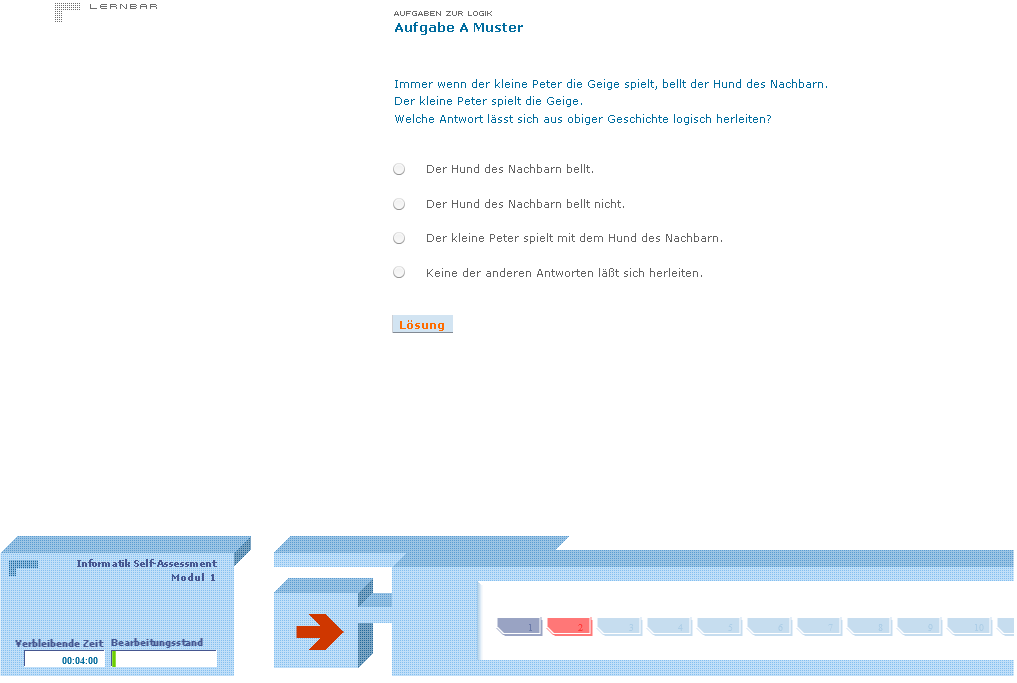
\includegraphics[width=\textwidth]{Jonas_Images/frankfurt1.png}
  \caption{}
  \label{fig:Bild1}
\end{figure*}
In Abbildung~\ref{fig:Bild1} ist das Grundlayout des Tests von der Universität Frankfurt zu sehen. 
Das Layout ist sehr ähnlich zu unserem und beinhaltet die Frage mit ihren Antworten, einen Fortschrittsbalken, einen Next-Button und eine Zeitanzeige.

Auch ist es möglich Grafiken anzeigen zu lassen.
Der Test wird in verschiedene Kategorien eingegliedert, die wiederholbar sind. 
Bei unserem Test ist die Erstellung von Kategorien ebenfalls möglich, ein Mehrfachbeantwortung ist jedoch ausgeschlossen.

Abschließend bietet der Test der Universität Frankfurt eine Bewertung der beantworteten Fragen.
Anders als die Universität Frankfurt enthält unser Test insbesondere eine persönliche Beurteilung des Erstellers.
Diese diehnt als Abschließendes Feedback für die erbrachte Leistung des Nutzers im Test.

\subsection{Test der RWTH Aachen}
\begin{figure*}[htbp] 
  \centering
     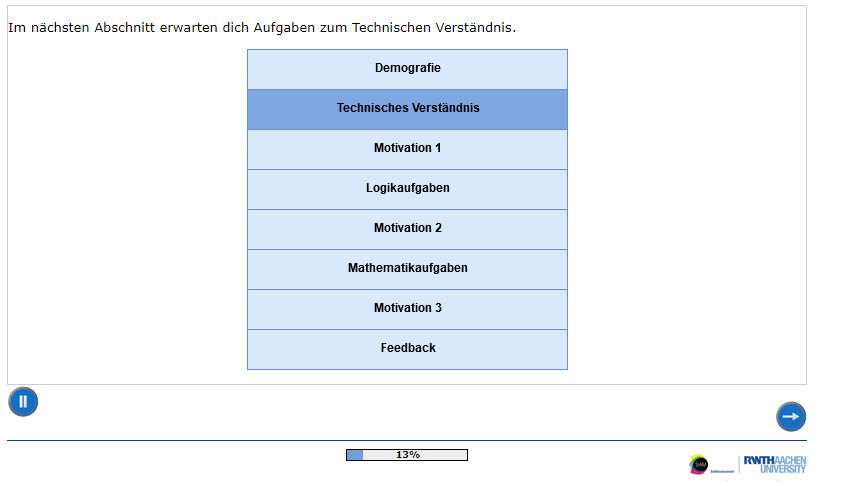
\includegraphics[width=0.5\textwidth]{Jonas_Images/Abschnitte.png}
  \caption{}
  \label{fig:Bild4}
\end{figure*}
Der Test der RWTH Aachen \footnote{\url{https://www.global-assess.rwth-aachen.de/rwth/tm_alt/}} ähnelt unserem Ansatz, wie man in Abbildung \ref{fig:Bild4} sehen kann.
Das Layout ist einfach gehalten und überschaubar. 
Es gibt einen Next-Button und einen Fortschrittsbalken.
In beiden Ansätzen besteht keine Möglichkeit, eine Frage zu überspringen.
Außerdem bedarf es einer Anmeldung, um am Test der Hochschule Aachen teilnehmen zu können.
Damit die Hemmschwelle zur Teilnahme möglichst niedrig gehalten wird, haben wir dafür entschieden, auf jede Form der Anmeldung zu verzichten.






\section{Architektur}
\label{Architektur}




\subsection{Creator}
\label{Julian}

Der 'Creator' wurde dazu entwickelt, um dem Benutzer die Möglichkeit zu geben, einen Self-Assesment-Test zu erstellen ohne die dafür anderweitig nötigen Programmierkenntnisse zu besitzen.
Das Programm verfügt über weitreichende Funktionen, damit ein vollständiger Test erstellt werden kann. 
In diesem Abschnitt werden diese Funktionen erläutert und eine Gesamtübersicht über diese Komponente gegeben. 

\subsubsection{Übersicht}
\begin{figure*}[htbp] 
  \centering
     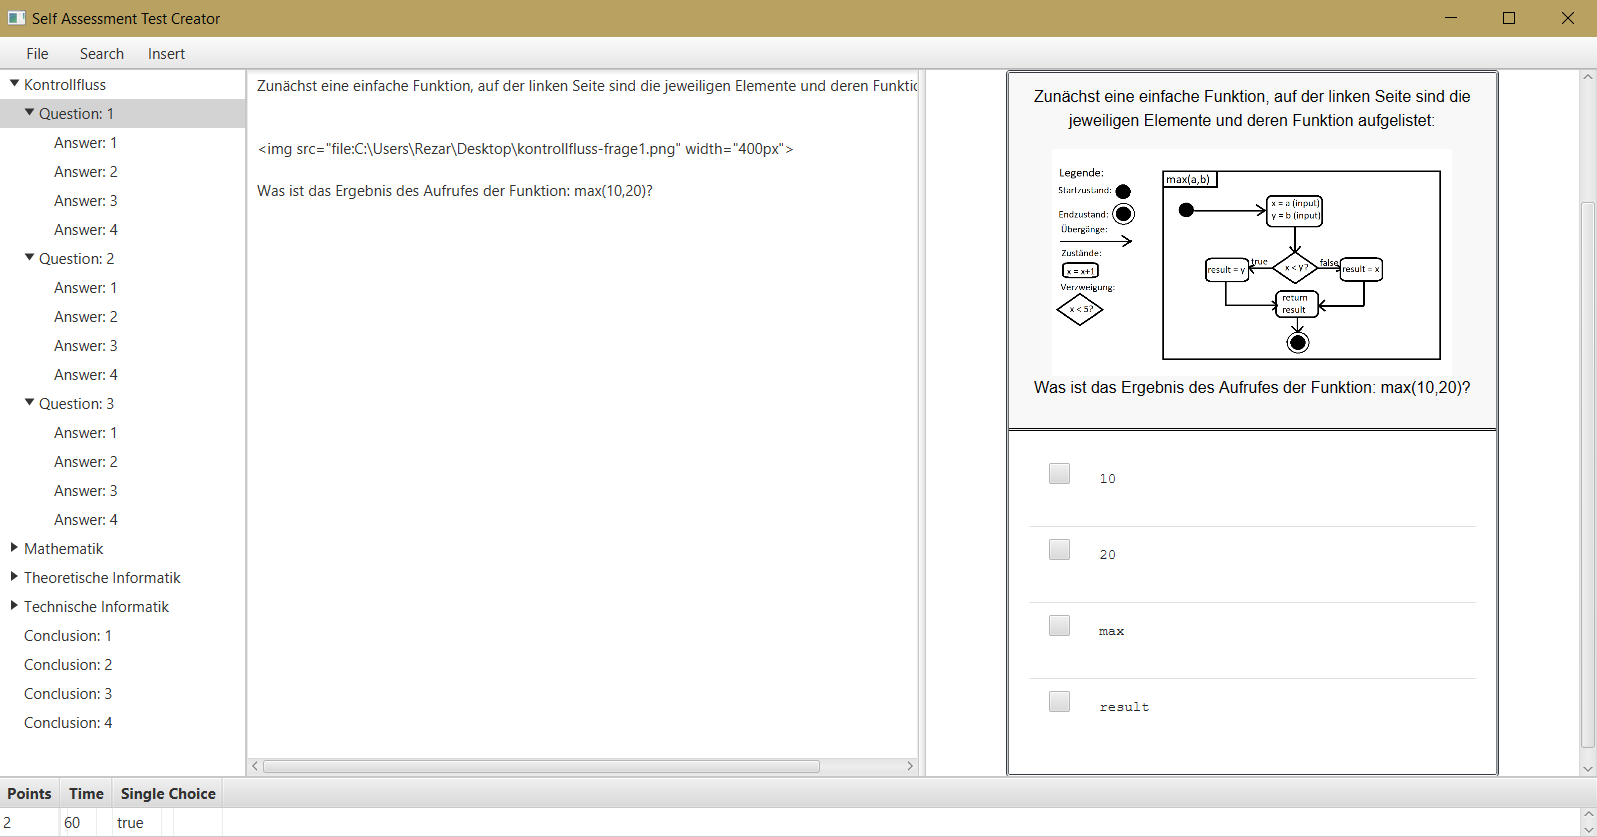
\includegraphics[width=\textwidth]{Julian_Images/Creator-Uebersicht.png}
  \caption{}
  \label{fig:Bild0}
\end{figure*}
Das Hauptfenster des 'Creators', zu sehen in Abbildung~\ref{fig:Bild0}, beinhaltet fünf wichtige Elemente die zur Übersicht und Erstellung des Tests dienen.
Auf der linken Seite ist ein 'TreeView'(A), der die Struktur des Testes darstellt.
In ihm werden die Kategorien, deren zugehörigen Fragen, Antworten und die Feedbacks angezeigt.
In jedem 'TreeItem' wird der Bezeichner des jeweiligen Objekts angezeigt.

Im Zentrum gibt es ein großes Textfeld (B), das den Inhalt des momentan ausgewählten 'TreeItems' wiedergibt.
Im Textfeld kann dieser Inhalt mithilfe von HTML und Markdown editiert werden.

Im unteren Bereich (C) wird eine Tabelle erstellt, die alle Attribute des im 'TreeView'  ausgewählten Elements anzeigt.
Kategorien besitzen als Attribut ihren Namen.
Fragen hingegen haben die Attribute Punkte und Zeit.
Verschiedenen Feebacks können hier verschiedene Punktebereiche zugeordnet werden.

Die obere Leiste (D) enthält 'MenuItems' mit mehreren Funktionen, die im nächsten Abschnitt näher betrachtet werden.

Auf der rechten Seite gibt es ein großes Vorschaufenster (E). 
Dieses zeigt eine Vorschau der gerade ausgewählten Frage an.


\subsubsection{Funktionen}
Unter der Option 'File' gibt es neun Buttons, die nach Funktionen sortiert sind. 
Die ersten vier, also 'New Category', 'New Question', 'New Answer' und 'New Conclusion', erstellen die jeweils zugehörigen Objekte.
'Delete Item' entfernt ein ausgewähltes Objekt.
Generate Website' erstellt einen Zip-Ordner, der die fertige Webseite enthält.
Mit 'Import XML' und 'Export XML' kann der Ersteller den bisherigen Forschritt in einer XML-Datei speichern, beziehungsweise einen bereits erstellten Test laden.
Das letzte 'MenuItem' 'Exit'  beendet das Programm.

Die zweite Option 'Insert' ist dazu da, Medien in Form von Bildern oder Videos in das Textfeld einzufügen. 
Dabei wird ein Medium eingefügt, indem der Ersteller den zugehörigen Dateinamen angibt.
 



\subsection{Parser}
\section{Tim's Abschnitt}\label{Tim}
\subsection{Hier kommt der erste Teil-Abschnitt }
bliBlaBlub\\
Die Architekturbeschreibugnsspraache Acme wurde von der ABLEGroup \cite{ABLEGroupHomePage-2018-10-12} entwickelt.


\subsection{Generator}
\label{Sokol}
Für das einfache Verwalten der Webseite, ist es vorgesehen, dass sie statisch ist.
In diesem Fall heißt das, dass es keinen Server geben soll, der dynamisch auf Anfragen des Benutzers reagiert.
Alle dynamischen Funktionen, wie das Laden neuer Fragen, finden auf der Benutzerebene statt.
Der Server liefert dem Benutzer bei Bedarf, also nur statische Dateien.

Der Vorteil dieses Designs ist, dass die Webseitendateien nur ein Mal aus den Java Objekten generiert werden müssen.
Für diese Funktion haben wir uns für die Template Engine Velocity \footnote{\url{http://velocity.apache.org/}} entschieden.

\subsubsection{Velocity}

Velocity erlaubt es Dokumente mit Variablen zu bestücken, die dann von Velocity mit dem Text aus den Java Objekten ersetzt werden.
Diese Dokumente werden Templates genannt.
Dafür werden Velocity das Java Objekt, der Name des Java Objektes in dem Tamplate und das Template an sich übergeben.
Velocity liest daraufhin das Template, sucht sich die Stellen heraus, die Variablen enthalten, und ersetzt diese mit den Inhalten des Java Objektes.

Ein Beispiel eines Velocity Templates ist in Listing~\ref{lst:velocity-example} gegeben.
Für das Beispiel wird angenommen, dass Velocity ein Question Objekt übergeben bekommt.
Dieses Question Objekt hat eine Funktion 'getContent()', die einen String zurückgibt, und eine andere Funktion 'getAnswers()', die eine Liste mit Answer Objekten zurückgibt.
Das Answer Objekt hat wiederum auch eine Funktion 'getContent()'.
Außerdem wird Velocity der Variablenname 'question' und das aufgeführte Template übergeben.

Das Zeichen '\$' in dem Template signalisiert Velocity, dass der danach kommende Text für Velocity vorgesehen ist.
So bemerkt Velocity, dass '\$question', das übergebene Question Objekt referenziert und ruft im ersten Fall die Funktion 'getContent()' auf.
Die Funktion wird ausgewertet und der zurückgegebene String wird an der Stelle des Funktionsaufrufs gesetzt.

Im Beispiel-Template sieht man auch eine 'foreach' Schleife, die mit '\#foreach' beginnt und mit '\#end' endet.
Diese Schleife sorgt dafür, dass der Abschnitt, der sich in der Schleife befindet, so oft geschrieben wird, wie es Answer Objekte in der von 'question.getAnswers()' zurückgegebenen Liste gibt.

Daraufhin wird '\$answer.getContent()' mit der entsprechenden Rückgabe der Answer Objektes ersetzt.


\begin{lstlisting}[basicstyle=\tiny,label={lst:velocity-example},caption={Beispiel eines Velocity Templates.},language=HTML]
<h1>$question.getContent()</h1>
<ul>
#foreach($answer in $question.getAnswers())
<li>$answer.getContent()</li>
#end
</ul>
\end{lstlisting}

\subsubsection{Erstellung der Webseite}
Für alle Dateien der Webseite, die Inhalte von den Java Objekten benötigen, wird eine Template Datei erstellt.
Daraufhin werden die ausgewerteten Templates, mit den anderen für die Webseite benötigten Dateien, in ein ZIP-Archiv gepackt und in einen von dem Benutzer des Generators festgelegten Ort gespeichert.

Um die Webseite dann zu veröffentlichen, müssen die Dateien im Archiv über einen HTTP-Server angeboten werden.





\subsection{Website}
\label{Jena}

Im folgenden soll skizziert werden, wie die Webseite des Online-Assessment-Tests bereitgestellt und präsentiert wird.
Dazu wird zunächst ein Überblick über die durch den Generator bereitgestellten statischen Dateien erstellt. Anschließend wird beschrieben, wie aus den statischen Daten die Seiten der Webseite zusammengestellt werden.
Ein besonderer Schwerpunkt liegt dabei auf der Anzeige der Fragen und der damit verbundenen Verwaltung des Zustandes.
Zuletzt wird die Auswertung und die Anzeige der Evaluierung des Tests beleuchtet.

\subsubsection{Überblick über die statischen Dateien}

Die im Abschnitt zuvor erwähnten statischen Dateien im durch den Generator erzeugten Zip-Archiv bestehen aus:

\begin{itemize}
\item einer einzelnen HTML-Seite, welche rudimentär mit zu ersetzenden Elementen gefüllt ist

\item den CSS-Dateien für das Styling der Seiten

\item den JavaScript-Dateien zur Manipulation der HTML-Seite 

\item den Fragen in Form von HTML und JSON-Dateien

\item und die im Text verwendeten Bilder und Videos
\end{itemize}

Die genannten Dateien werden anschließend mithilfe eines HTTP-Servers dem Client angeboten. 

\subsubsection{Anzeige der Fragen}

Die gesamte Webseite basiert auf einer einzelnen HTML-Seite, die für jede Frage des Tests verändert wird.
Ist im folgenden die Rede von einer Seite, so wird damit entsprechend die manipulierte HTML-Seite für eine Frage referenziert.

Im folgenden soll der Aufbau jeder Fragenseite, von oben nach unten betrachtet und erläutert werden. 
Die Seiten beginnen stets mit dem Logo der Universität Stuttgart. 
Es folgt eine Übersichtsleiste (A), welche die verschiedenen Kategorien des Tests anzeigt. 
Die Kategorie der aktuell angezeigten Frage wird zur Hervorhebung grau markiert. 

Unterhalb der Übersichtsleiste findet sich der Fortschrittsbalken (B). 
Dieser setzt sich aus $n$ kleineren Balken zusammen, wobei $n$ die Gesamtanzahl aller Fragen ist.
Die Anzahl der gefüllten Balken gibt dabei an, wie viele Fragen, inklusive der aktuellen Frage, bisher beantwortet wurden, die Anzahl der leeren Balken stellt dagegen die verbleibende Anzahl an Frage dar. 

Unterhalb des Fortschrittsbalkens und zentral im Sichtfeld werden die aktuelle Frage und ihre Antwortmöglichkeiten angezeigt. 
Die Frage erhält ein eigenes Feld (C), in welcher optional eine Erklärung zur Frage und ein Bild angezeigt werden können.
Separiert von der Frage folgen dann ihre Antwortmöglichkeiten (D), die jeweils eigene Felder erhalten. 
Für alle Fragen wird links neben jeder Antwort eine Checkbox platziert.
Hierbei können Antworten auch Bilder beinhalten.

Zuletzt findet sich der Next-Button (E) rechtsbündig unter dem Feld der Frage und ihrer Antworten, mit welchem die nächste Frage anzeigen lässt.

Es wird zunächst die nahezu leere HTML-Seite aufgerufen, welche als Hülle für die Seiten der Fragen dient. 
In der Folge wird der Inhalt der HMTL-Seite durch die aktuell anzuzeigende Frage bestimmt.

Für jede Frage des Online-Assessment-Tests wird das Codefragment, welches zur Anzeige der Frage benötigt wird, aus der serverseitig gespeicherten HTML-Datei der Frage gelesen und in das HTML-Dokument geschrieben. 
Zusätzlich legt eine JSON-Datei pro Frage das optionale Zeitlimit und die Punkte für die korrekte Beantwortung der Frage fest.

Die bisher angezeigten und beantworteten Fragen werden im Rahmen der Zustandsverwaltung mitverwaltet, die aktuelle Frage wird dann anhand des Zustands abgeleitet.

\subsubsection{Zustandsverwaltung}

Der Zustand der Webseite setzt sich im wesentlichen aus den bisher beantworteten Fragen und ihren Antwortmöglichkeiten zusammen. 
Für jede beantwortete Frage wird ein Bitstring der Länge $m$ verwaltet. Dieser gibt an, wie viele Antwortmöglichkeiten die Frage aufweißt und wie die Frage durch den Nutzer beantwortet wurde. 
Die Anzahl der Antwortmöglichkeiten einer Frage wird in den ersten $5$ Bit des Bitstrings kodiert. 
Die restlichen $m - 5$ Bit des Bitstrings stellen die einzelnen Antwortmöglichkeiten der Frage dar. Jede einzelne Antwortmöglichkeit wird dabei durch ein einzelnes Bit repräsentiert, welches genau dann gesetzt ist, wenn die Antwortmöglichkeit angekreuzt wurde.
Wird beispielsweise eine Frage mit $3$ Antwortmöglichkeiten gestellt, wobei nur die erste der drei Antwortmöglichkeiten angekreuzt wurde, so ist der resultierende Bitstring der Länge $8$ für diese Frage $00011100$.

Die einzelnen Bitstrings der jeweiligen Fragen werden dann konkateniert und der resultierende String durch die Umwandlung in \textit{Base64} verkürzt. 
Anschließend wird diese Zeichenfolge als URL-Parameter an die aktuelle URL angehängt.
 
Für die Anzeige einer Frage wird somit die aktuelle URL abgerufen, der URL-Parameter extrahiert und dekodiert.
Aus dem dekodierten Bitstring wird dann die Anzahl bisher beantworteter Fragen errechnet und anhand dessen die HTML und JSON-Datei der aktuellen Frage abgeleitet.

Beim initialen Aufruf der Webseite wird somit die erste Frage angezeigt, wobei der URL-Parameter leer ist.
Beim Drücken des Next-Buttons werden dann die Antworten ausgewertet, ehe das Skript zur Verwaltung des Zustandes mit dem Ergebnis aufgerufen wird. 
Die URL wird dann entsprechend angepasst und die nächste Frage geladen.

\subsubsection{Evaluierung}

Wurde die letzte Frage erreicht und der Next-Button gedrückt, wird der finale Zustand aus der URL gelesen.
Anschließend wird das Skript zur Auswertung der Evaluation aufgerufen. 
Dieses Skript vergleicht die Antworten des Nutzers mit einem durch den Generator bereitgestellten Lösungsstring.
Für jede korrekt beantwortete Frage wird die durch die Frage vergebene Punktzahl zur erreichten Kategoriepunktzahl und Gesamtpunktzahl addiert.
Die Kategoriepunktzahl gibt die erreichte Punktzahl für sämtliche Fragen einer Kategorie an, die Gesamtpunktzahl die erreichte Punktzahl für die Gesamtheit aller Fragen.

Die verschiedenen Kategoriepunktzahlen und die Gesamtpunktzahl werden dann in einer spezifischen Evaluationsseite dargestellt wird.
 
Abbildung Z zeigt die Evaluation nach einem Durchlauf eines Beispieltests. 

Die Evaluationsseite setzt sich aus der Anzeige der erreichten Punkte für jede einzelne Kategorie und einem Fazit abhängig von der Gesamtpunktzahl zusammen.
Für die einzelnen Kategorien wird anhand eines Fortschrittsbalkens angezeigt, wie viele der maximal erreichbaren Punkte der betroffenen Kategorie erreicht wurden. 

Für das Fazit wird eine spezifische JSON-Datei anhand der erreichten Gesamtpunktzahl ausgewertet. 
Der Ersteller des Tests legt in dieser Datei fest, welcher Fazittext für welches Punkteintervall angezeigt werden soll. 
Es wird dann überpürft in welchem Intervall die erreichte Gesamtpunktzahl liegt und das entsprechende Fazit im Dropdown-Feld unter den Fortschrittsbalken angezeigt. 



\section{Anwendungsszenario}
\subsection{Programm ausführen}
Zuerst führt man die Datei \textit{TextEditor.java} aus, die wie folgt im Projekt-Ordner zu finden ist:\newline 

\textit{src>>main>>java>>creator>>TextEditor.java}\newline 

Jetzt öffnet sich das Haupt-Fenster des Creators (siehe Abbildung \ref{fig:Bild0}).
\subsection{Fragen hinzufügen}
Nun fügen wir unter File in der Toolbar neue Kategorien mit Fragen und deren Antworten hinzu. Dabei geben wir an, wie viele Punkte eine Antwort gibt, wie viel Zeit sie maximal beötigt, und ob sie Single Choice zulässt an (Abbildung \ref{fig:Bild0}). Nachdem wir angegeben haben welche Anworten korrekt sind, fügen wir noch entsprechende Conclusions hinzu, deren Range angibt, bis zu wie vielen Punkten jene Conclusion am Ende in der Bewertung angezeigt wird. 
\subsection{Webseite generieren}
Falls wir noch nicht fertig sind und eine Pause machen möchten, kann unser Fortschritt als XML-Datei export und zu einem späteren Zeitpunkt wieder importiert werden.\newline Um die letztendliche HTML-Datei zu erstellen clickt man als Nächstes auf \textit{Generate Website} unter \textit{File} und speichert das Projekt mit der inkludierten HTML-Datei in einem beliebigen Ordner.
\subsubsection*{\textit{optional: lokalen Server erstellen}}
Da der Selfassessment-Test einen Server benötigt, kann man, falls man keinen Server besitzt, auch das Ganze auf einem Lokalen Server testen. Dies gelingt zum Beispiel mit \textit{Node.js}.
\subsection{Selfasessment-Test durchführen}
Sobald die Verbindung zu einem Server besteht, kann der Test benutzt werden. Der Test an sich ist sehr intuitiv zu bedienen. Man wählt seine Antworten aus und clickt auf \textit{Next}. Sollte der Timer ablaufen wird die eingeloggte Antwort genommen und zur nächsten Frage gesprungen. Am Ende kann man noch seine Bewertung einsehen.

\section{Zusammenfassung und Ausblick}

\onecolumn
% einfacher Zeilenabstand
\singlespacing
% Literaturliste soll im Inhaltsverzeichnis auftauchen
\newpage
\addcontentsline{toc}{section}{Literaturverzeichnis}
% Literaturverzeichnis anzeigen
\renewcommand\refname{Literaturverzeichnis}

\bibliography{Hauptdatei}
\end{document}